\documentclass[10pt]{beamer}

\usetheme[progressbar=frametitle]{metropolis}
\usepackage{appendixnumberbeamer}
\usepackage{amsmath}
\usepackage{booktabs}
\usepackage[scale=2]{ccicons}

\usepackage{pgfplots}
\usepgfplotslibrary{dateplot}

\usepackage{xspace}
\usepackage{tcolorbox}
\newcommand{\themename}{\textbf{\textsc{metropolis}}\xspace}
\definecolor{darkred}{RGB}{173,34,48}

\title{Scattering Amplitudes as Differential Forms}
\subtitle{}
% \date{\today}
\date{}
\author{Chi Zhang}
\institute{Institute of Theoretical Physics}
% \titlegraphic{\hfill\includegraphics[height=1.5cm]{logo.pdf}}

\begin{document}

\maketitle

\iffalse
\begin{frame}{Table of contents}
  \setbeamertemplate{section in toc}[sections numbered]
  \tableofcontents[hideallsubsections]
\end{frame}

\section{Introduction}

\begin{frame}[fragile]{Metropolis}

  The \themename theme is a Beamer theme with minimal visual noise
  inspired by the \href{https://github.com/hsrmbeamertheme/hsrmbeamertheme}{\textsc{hsrm} Beamer
  Theme} by Benjamin Weiss.

  Enable the theme by loading

  \begin{verbatim}    \documentclass{beamer}
    \usetheme{metropolis}\end{verbatim}

  Note, that you have to have Mozilla's \emph{Fira Sans} font and XeTeX
  installed to enjoy this wonderful typography.
\end{frame}
\begin{frame}[fragile]{Sections}
  Sections group slides of the same topic

  \begin{verbatim}    \section{Elements}\end{verbatim}

  for which \themename provides a nice progress indicator \ldots
\end{frame}

\section{Background}
\fi
\begin{frame}{Background}
$\mathcal{N}=4$ Supersymmetric Yang-Mills theory
\begin{itemize}
  \item AdS/CFT Duality
  \item Integrability
  \item Twistor strings
  \item Amplituhderon/Grassmaniann
  \item Lots of Math
\end{itemize}
\end{frame}

\begin{frame}
The content of $\mathcal{N}=4$ SYM: 
\begin{itemize}
  \item 2 gauge bosons with $h=\pm1$: \quad$\vert a \rangle^{+1}$, $\vert a \rangle^{-1}_{IJKL}$
  \item 8 fermions with $h=\pm\frac{1}{2}$:\qquad\quad\:\:$\vert a \rangle^{+1/2}_{I}$,$\vert a \rangle^{-1/2}_{IJK}$
  \item {6 spinless scalars}:  \qquad\qquad\qquad\:\!$\vert a \rangle^{0}_{IJ}$
  \end{itemize}
They are all related by supersymmetric generators $Q_{I=1,2,3,4}^{\alpha}$ and $\tilde{Q}_{I=1,2,3,4}^{\dot{\alpha}}$. For example, $\vert a \rangle^{+1/2}_{I}=\tilde{Q}_{I}\vert a \rangle^{+1}$。 \\Thus, all on-shell states in $\mathcal{N}=4$ SYM can be grouped into a \emph{single} supermultiplet:
\begin{align*}
  \vert a\rangle &\equiv \exp(\tilde{Q}_{I}\cdot\tilde{\lambda}\cdot\tilde{\eta}^{I})\vert a\rangle^{+1} \\
  &= \vert a \rangle^{+1}+\tilde{\eta}^{I}\vert a\rangle_{I}^{1/2}+\cdots+\frac{1}{4!}\tilde{\eta}^{I}\tilde{\eta}^{J}\tilde{\eta}^{K}\tilde{\eta}^{L}\vert a \rangle^{-1}_{IJKL}
\end{align*} 
\end{frame}




\begin{frame}

  \begin{alertblock}{Superamplitudes, not amplitudes!}
    \phantom{af}\\
    \begin{align*}
      &\mathcal{A}_{n,\text{tree}}^{k=2}=\frac{\delta^{4}(P)\delta^{8}(Q)}{\langle 12\rangle\cdots\langle n1\rangle} \\
      &\mathcal{A}_{n,\text{tree}}^{k=3}=\mathcal{A}_{n,\text{tree}}^{k=2} \sum_{2<i<j<n-1}[1,i{-}1,i,j,j{+}1] \:(\textbf{\scriptsize{Momentum Twistor come in!}})\\
      &\mathcal{A}_{n,\text{tree}}^{k}\text{ are known for any n and any k} \\
      &\mathcal{A}_{n,L=1}^{k}\text{ are known for any n and any k} \\
      &\mathcal{A}_{n,L=2}^{k}\text{ are known for any n and k=2} \\ 
      &\cdots \\
      &\mathcal{A}_{6,5}^{2} \text{ are known.} 
    \end{align*}
  \end{alertblock}
  \\
  \footnotesize{\textcolor{darkred}{[Bern, Caron-Huot, Dixon, Drummond, Duhr, Foster, Gürdo˘ gan, He, Henn, von Hippel, Golden,
   Kosower, Papathanasiou, Pennington, Roiban, Smirnov, Spradlin, Vergu, Volovich, ...]}}
\end{frame}

\begin{frame}{Amplituhderon \& Positive geometry}

  Positive geometry is defined by its boundary which also is a \emph{positive geometry}. For each positive geometry, we define a canonical form  such that it only has logarithmic residues on its boundary.
  For example:
  \begin{tcolorbox}
  \begin{align*}
    &\Omega[\{0<x<1\}]=\frac{dx}{x}-\frac{dx}{x-1}=d\log\frac{x}{1-x}\\
    &\Omega[\{0<x<y<1\}]=d\log\frac{x}{x-y}\wedge d\log\frac{x-y}{1-y}\\
    &\Omega[\{x_{ij}z_{ij}+y_{ij}w_{ij}<0\vert 1\leq i<j\leq L\}] = \text{4pt L-loop planar integrand!} 
  \end{align*} 
\end{tcolorbox}
\\
  Amplituhderon is a positive geometry defined in Momentum twistor space. \\
  \footnotesize{\textcolor{darkred}{[Arkani-Hamed, Bai, Thomas, Trnka,$\cdots$ ]}}
\end{frame}


\begin{frame}{Motivation}
\begin{itemize}[<+->]
  \item  Motivation: Try to define the Amplituhderon in terms of usual spinor-helicity variables $\{\lambda_{i},\tilde{\lambda}_{i}\}$ 
  \item It is too ambitious. Find the canonical form first.
  \item Method: Combine different particles by $d\lambda,d\tilde{\lambda}$ in place of $\eta_{I}$
   \begin{equation*}
    \vert a\rangle
     = (d\lambda)^{2}\vert a \rangle^{+1}+\cdots+(d\tilde{\lambda})^{2}\vert a\rangle^{-1}
  \end{equation*}
   \item The result of this simple replacement is \\
  \emph{every amplitude with n-point and L-loop turn out to be} $(2n-4+4L)$-$d\log$ form  
  \end{itemize}
   
\end{frame}

\begin{frame}{MHV case}
  some simple examples:
  \begin{align*}
    \Omega_{3,\text{MHV}}&=d\log\frac{\langle 12\rangle}{\langle 23\rangle}\wedge d\log\frac{\langle 23\rangle}{\langle 13\rangle}   \\ 
    \Omega_{4,\text{MHV}}&=d\log\frac{\langle 12\rangle}{\langle 23\rangle}\wedge d\log\frac{\langle 23\rangle}{\langle 13\rangle} \wedge 
    d\log\frac{\langle 13\rangle}{\langle 34\rangle}\wedge d\log\frac{\langle 34\rangle}{\langle 14\rangle} 
  \end{align*}
  The result for MHV n-pt corresponds to a triangulation of $n$-gon :
  \begin{equation*}
    \Omega_{n,\text{MHV}} = \bigwedge_{i=1}^{n-2} d\log\frac{\langle a_{i}b_{i}\rangle}{\langle b_{i}c_{i}\rangle}\wedge d\log\frac{\langle b_{i}c_{i}\rangle}{\langle a_{i}b_{i}\rangle}
  \end{equation*}
  \begin{equation*}
    \raisebox{-1.0cm}{
    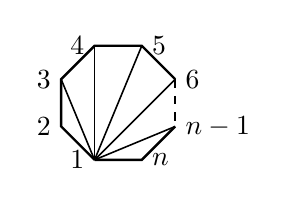
\begin{tikzpicture}[scale=0.3]
    \draw[line width=.03cm]  (0,0) coordinate (1) node [left=0pt]{1}
      --++(135:2) coordinate (2) node [left=0pt]{2}
      --++(90:2) coordinate (3) node [left=0pt]{3}
      --++(45:2) coordinate (4) node [left=0pt]{4}
      --++(0:2) coordinate (5) node [right=0pt]{5}
      --++(-45:2) coordinate (6) node [right=0pt]{6}
      ++(-90:2) coordinate (7) node [right=0pt]{$n-1$}
      --++(-135:2) coordinate (8) node [right=0pt]{$n$}
      --+(180:2);
      \draw[line width=.03cm,dashed] (6)--(7);
      \draw[line width=.02cm] (1)--(3);
      \draw[line width=.02cm] (1)--(4);
      \draw[line width=.02cm] (1)--(5);
      \draw[line width=.02cm] (1)--(6);
      \draw[line width=.02cm] (1)--(7);
    \end{tikzpicture}}
    = \bigwedge_{i=2}^{n-1} d\log \frac{\langle1\,i\rangle}{\langle i+1\, 1\rangle}\wedge d\log \frac{\langle i\, i+1\rangle}{\langle i+1\, 1\rangle} \:.
    \end{equation*} 
\end{frame}

\begin{frame}{NMHV case}
  \begin{align*}
    &\sum_{1<i<j<n}
    \raisebox{-1.0cm}{
    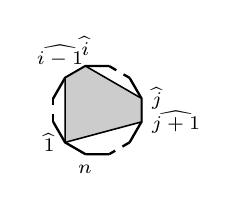
\begin{tikzpicture}[scale=0.15]
       \draw[line width=.03cm]  (0,0) coordinate (12) node [left=0.2pt,below=0.1pt]{\scriptsize$n$}
      --++(150:2) coordinate (1) node [left=0pt]{\scriptsize$\widehat{1}$}
      --++(120:2) coordinate (2)
      ++(90:2) coordinate (3)
      --++(60:2) coordinate (4) node [above=0.3pt]{\scriptsize$\widehat{i-1}\:\:$}
      --++(30:2) coordinate (5) node [left=0.1pt,above=0.1pt]{\scriptsize$\widehat{i}$}
      --++(00:2) coordinate (6)
      ++(-30:2) coordinate (7)
      --++(-60:2) coordinate (8) node [right=0pt,]{\scriptsize$\widehat{j}$}
      --++(-90:2) coordinate (9) node [right=0pt]{\scriptsize$\widehat{j+1}$}
      --++(-120:2) coordinate (10)
      ++(-150:2) coordinate (11)
      --+(180:2);
      \fill[black!20] (1)--(4)--(5)--(8)--(9)--(1);
      \draw[line width=.02cm] (1)--(4)--(5)--(8)--(9)--(1);
      \draw[line width=.03cm,dashed] (2)--(3);
      \draw[line width=.03cm,dashed] (6)--(7);
      \draw[line width=.03cm,dashed] (10)--(11);
    \end{tikzpicture}
    }
    =\sum_{1<i<j<n} \Omega_{\text{MHV}}(1,\cdots ,i-1)\wedge  \Omega_{\text{MHV}}(i,\cdots,j)
    \nonumber \\
    &\quad \wedge \Omega_{\text{MHV}}(j+1,\cdots ,n,1)\wedge  \Omega_{\overline{\text{MHV}}}(\widehat{1},\widehat{i-1},\widehat{i},\widehat{j},\widehat{j+1}) \:,\label{NMHV}
    \end{align*}
    where 
\begin{align*}
\tilde{\lambda}_{\hat{1}} &=\tilde{\lambda}_{1}+\sum_{a=2}^{i-1}\frac{%
\langle i\,  a\rangle }{\langle i\,  1\rangle }\tilde{\lambda}_{a}+\sum_{a=j+2}^{n}%
\frac{\langle a\,  j+1\rangle }{\langle 1\,  j+1\rangle }\tilde{\lambda}_{a}\:, \\
\tilde{\lambda}_{\hat{i}} &=\tilde{\lambda}_{i}+\sum_{a=2}^{i-1}\frac{%
\langle a\,  1\rangle }{\langle i\,  1\rangle }\tilde{\lambda}_{a} \:, \qquad
\tilde{\lambda}_{\widehat{i+1}} =\tilde{\lambda}_{i+1}+\sum_{a=i+2}^{j-1}%
\frac{\langle j\,  a\rangle }{\langle j\,  i+1\rangle }\tilde{\lambda}_{a} \:,\\
\tilde{\lambda}_{\hat{j}} &=\tilde{\lambda}_{j}+\sum_{a=m+1}^{n-1}%
\frac{\langle a\,  i+1\rangle }{\langle j\,  i+1\rangle }\tilde{\lambda}_{a} \:, \qquad
\tilde{\lambda}_{\widehat{j+1}} =\tilde{\lambda}_{j+1}+\sum_{a=m+1}^{n-1}%
\frac{\langle 1\,  a\rangle }{\langle 1\,  j+1\rangle }\tilde{\lambda}_{a} \:.
\end{align*}
    There is an algorithm to obtain $\Omega_{n,k}^{\text{tree}}$
\end{frame}


\begin{frame}
\begin{itemize}[<+->]
  \item The obstacle to its geometry is the dimension.
  \item Recently, Cachazo \emph{et al.} find the canonical form for MHV case can be written as
  \begin{align*}
    \Omega_{n,\text{MHV}}&=\frac{1}{(n-2)!} \left(\sum_{i=2}^{n-1} d\log \frac{\langle1\,i\rangle}{\langle i+1\, 1\rangle}\wedge d\log \frac{\langle i\, i+1\rangle}{\langle i+1\, 1\rangle}\right)^{n-2} \\
    &\sim \frac{1}{(n-2)!} \left(\text{canonical form for $n$-gon})^{n-2}
  \end{align*}  
\end{itemize}
\end{frame}


\begin{frame}{Outlook}
  \begin{itemize}
    \item The connection with amplituhderon $4k$-form.
    \item How to intrinsically define amplituehdron in momentum space.
    \item Generalization to loop level and more general theories. 
  \end{itemize}  
\end{frame}

\iffalse
\section{Titleformats}

\begin{frame}{Metropolis titleformats}
	\themename supports 4 different titleformats:
	\begin{itemize}
		\item Regular
		\item \textsc{Smallcaps}
		\item \textsc{allsmallcaps}
		\item ALLCAPS
	\end{itemize}
	They can either be set at once for every title type or individually.
\end{frame}

{
    \metroset{titleformat frame=smallcaps}
\begin{frame}{Small caps}
	This frame uses the \texttt{smallcaps} titleformat.


\end{frame}
}

{
\metroset{titleformat frame=allsmallcaps}
\begin{frame}{All small caps}
	This frame uses the \texttt{allsmallcaps} titleformat.

	\begin{alertblock}{Potential problems}
		As this titleformat also uses smallcaps you face the same problems as with the \texttt{smallcaps} titleformat. Additionally this format can cause some other problems. Please refer to the documentation if you consider using it.

		As a rule of thumb: Just use it for plaintext-only titles.
	\end{alertblock}
\end{frame}
}

{
\metroset{titleformat frame=allcaps}
\begin{frame}{All caps}
	This frame uses the \texttt{allcaps} titleformat.

	\begin{alertblock}{Potential Problems}
		This titleformat is not as problematic as the \texttt{allsmallcaps} format, but basically suffers from the same deficiencies. So please have a look at the documentation if you want to use it.
	\end{alertblock}
\end{frame}
}

\section{Elements}

\begin{frame}[fragile]{Typography}
      \begin{verbatim}The theme provides sensible defaults to
\emph{emphasize} text, \alert{accent} parts
or show \textbf{bold} results.\end{verbatim}

  \begin{center}becomes\end{center}

  The theme provides sensible defaults to \emph{emphasize} text,
  \alert{accent} parts or show \textbf{bold} results.
\end{frame}

\begin{frame}{Font feature test}
  \begin{description} [<+->]
    \item Regular
    \item \textit{Italic} 
  \end{description}
\end{frame}

\begin{frame}{Lists}
  \begin{columns}[T,onlytextwidth]
    \column{0.33\textwidth}
      Items
      \begin{itemize}
        \item Milk \item Eggs \item Potatos
      \end{itemize}

    \column{0.33\textwidth}
      Enumerations
      \begin{enumerate}
        \item First, \item Second and \item Last.
      \end{enumerate}

    \column{0.33\textwidth}
      Descriptions
      \begin{description}
        \item[PowerPoint] Meeh. \item[Beamer] Yeeeha.
      \end{description}
  \end{columns}
\end{frame}
\begin{frame}{Animation}
  \begin{itemize}[<+- | alert@+>]
    \item \alert<4>{This is\only<4>{ really} important}
    \item Now this
    \item And now this
  \end{itemize}
\end{frame}
\begin{frame}{Figures}
  \begin{figure}
    \newcounter{density}
    \setcounter{density}{20}
    \begin{tikzpicture}
      \def\couleur{alerted text.fg}
      \path[coordinate] (0,0)  coordinate(A)
                  ++( 90:5cm) coordinate(B)
                  ++(0:5cm) coordinate(C)
                  ++(-90:5cm) coordinate(D);
      \draw[fill=\couleur!\thedensity] (A) -- (B) -- (C) --(D) -- cycle;
      \foreach \x in {1,...,40}{%
          \pgfmathsetcounter{density}{\thedensity+20}
          \setcounter{density}{\thedensity}
          \path[coordinate] coordinate(X) at (A){};
          \path[coordinate] (A) -- (B) coordinate[pos=.10](A)
                              -- (C) coordinate[pos=.10](B)
                              -- (D) coordinate[pos=.10](C)
                              -- (X) coordinate[pos=.10](D);
          \draw[fill=\couleur!\thedensity] (A)--(B)--(C)-- (D) -- cycle;
      }
    \end{tikzpicture}
    \caption{Rotated square from
    \href{http://www.texample.net/tikz/examples/rotated-polygons/}{texample.net}.}
  \end{figure}
\end{frame}
\begin{frame}{Tables}
  \begin{table}
    \caption{Largest cities in the world (source: Wikipedia)}
    \begin{tabular}{lr}
      \toprule
      City & Population\\
      \midrule
      Mexico City & 20,116,842\\
      Shanghai & 19,210,000\\
      Peking & 15,796,450\\
      Istanbul & 14,160,467\\
      \bottomrule
    \end{tabular}
  \end{table}
\end{frame}
\begin{frame}{Blocks}
  Three different block environments are pre-defined and may be styled with an
  optional background color.

  \begin{columns}[T,onlytextwidth]
    \column{0.5\textwidth}
      \begin{block}{Default}
        Block content.
      \end{block}

      \begin{alertblock}{Alert}
        Block content.
      \end{alertblock}

      \begin{exampleblock}{Example}
        Block content.
      \end{exampleblock}

    \column{0.5\textwidth}

      \metroset{block=fill}

      \begin{block}{Default}
        Block content.
      \end{block}

      \begin{alertblock}{Alert}
        Block content.
      \end{alertblock}

      \begin{exampleblock}{Example}
        Block content.
      \end{exampleblock}

  \end{columns}
\end{frame}
\begin{frame}{Math}
  \begin{equation*}
    e = \lim_{n\to \infty} \left(1 + \frac{1}{n}\right)^n
  \end{equation*}
\end{frame}
\begin{frame}{Line plots}
  \begin{figure}
    \begin{tikzpicture}
      \begin{axis}[
        mlineplot,
        width=0.9\textwidth,
        height=6cm,
      ]

        \addplot {sin(deg(x))};
        \addplot+[samples=100] {sin(deg(2*x))};

      \end{axis}
    \end{tikzpicture}
  \end{figure}
\end{frame}
\begin{frame}{Bar charts}
  \begin{figure}
    \begin{tikzpicture}
      \begin{axis}[
        mbarplot,
        xlabel={Foo},
        ylabel={Bar},
        width=0.9\textwidth,
        height=6cm,
      ]

      \addplot plot coordinates {(1, 20) (2, 25) (3, 22.4) (4, 12.4)};
      \addplot plot coordinates {(1, 18) (2, 24) (3, 23.5) (4, 13.2)};
      \addplot plot coordinates {(1, 10) (2, 19) (3, 25) (4, 15.2)};

      \legend{lorem, ipsum, dolor}

      \end{axis}
    \end{tikzpicture}
  \end{figure}
\end{frame}
\begin{frame}{Quotes}
  \begin{quote}
    Veni, Vidi, Vici
  \end{quote}
\end{frame}

{%
\setbeamertemplate{frame footer}{My custom footer}
\begin{frame}[fragile]{Frame footer}
    \themename defines a custom beamer template to add a text to the footer. It can be set via
    \begin{verbatim}\setbeamertemplate{frame footer}{My custom footer}\end{verbatim}
\end{frame}
}

\begin{frame}{References}
  Some references to showcase
\end{frame}

\section{Conclusion}

\begin{frame}{Summary}

  Get the source of this theme and the demo presentation from

  \begin{center}\url{github.com/matze/mtheme}\end{center}

  The theme \emph{itself} is licensed under a
  \href{http://creativecommons.org/licenses/by-sa/4.0/}{Creative Commons
  Attribution-ShareAlike 4.0 International License}.

  \begin{center}\ccbysa\end{center}

\end{frame}

{\setbeamercolor{palette primary}{fg=black, bg=yellow}
\begin{frame}[standout]
  Questions?
\end{frame}
}

\appendix

\begin{frame}[fragile]{Backup slides}
  Sometimes, it is useful to add slides at the end of your presentation to
  refer to during audience questions.

  The best way to do this is to include the \verb|appendixnumberbeamer|
  package in your preamble and call \verb|\appendix| before your backup slides.

  \themename will automatically turn off slide numbering and progress bars for
  slides in the appendix.
\end{frame}

\begin{frame}[allowframebreaks]{References}

  \bibliography{demo}
  \bibliographystyle{abbrv}

\end{frame}

\fi
\end{document}
